\documentclass{beamer}
%\let\Tiny=\tiny
\usepackage{amsmath,amsthm,amssymb,amsfonts,enumerate,epsfig,ulem,wrapfig}
\usepackage[utf8]{inputenc}
\usepackage[spanish]{babel}
\usepackage{graphicx}
\usepackage{beamerthemesplit}
\usepackage{cancel}

% Theorem styles
\newtheorem{exa}{Ejemplo}
\renewenvironment{example}{\begin{exa}}{\end{exa}} 

\newtheorem{defi}{Definición}
\renewenvironment{definition}{\begin{defi}}{\end{defi}}

\newtheorem{teo}{Teorema}
\renewenvironment{theorem}{\begin{teo}}{\end{teo}}


% Usual numerical systems
\newcommand{\N}{{\ensuremath{\mathbb{N}}}}
\newcommand{\Z}{{\ensuremath{\mathbb{Z}}}}
\newcommand{\Q}{{\ensuremath{\mathbb{Q}}}}
\newcommand{\R}{{\ensuremath{\mathbb{R}}}}
\newcommand{\C}{{\ensuremath{\mathbb{C}}}}

\newcommand{\stframe}[1]{\begin{frame} \begin{center}\Large{\textbf{{#1}}}\end{center}\end{frame}}


%\usetheme{Rochester}
%\usetheme{Malmoe}
%\setbeamertemplate{navigation symbols}{} 
%\useoutertheme{infolines}

\title[Sistemas Dinámicos Planos]{Sistemas Dinámicos Planos}
\institute[UNAL]{Universidad Nacional de Colombia \\ Medellín \\ \texttt{jatorreshen@unal.edu.co}}
\author{Jorge A. Torres H.}
\date{22 de abril de 2013}

\begin{document}

% titulo
\begin{frame}[plain]
    \titlepage
\end{frame}

% Introducción
\section{Conceptos Básicos}
\stframe{Conceptos Básicos}

\begin{frame}{Sistemas Dinámicos}
Los \textbf{sistemas dinámicos} surgen al tratar de especificar mediante un modelo matemático procesos en los que es posible describir la dependencia en el tiempo de un punto en un espacio geométrico mediante la aplicación de una fórmula o ``regla''.
\end{frame}

\begin{frame}{Sistemas Dinámicos}
Los sistemas dinámicos aparecen con naturalidad en virtualmente todas las áreas de la ciencia: pueden modelar el movimiento de un sistema mecánico, la cantidad de individuos a través del tiempo de una población de peces en un lago, fenómenos relacionados con procesos químicos en los que hay intercambio de materia e inclusive en la predicción del clima.
\end{frame}

\begin{frame}{Sistemas Dinámicos}
La clave para esta unificación se encuentra en el concepto de ``estado'' y ``regla de evolución'': un sistema, en un instante de tiempo dado, se encuentra en algún estado posible, representado generalmente como un punto en el espacio euclídeo $\R^n$. La regla de evolución del sistema es una regla fija (función) que determina el estado futuro de dicho punto.
\end{frame}

\begin{frame}{¿Por qué estudiar sistemas dinámicos planos?}
Limitarse a sistemas planos definidos en $\R^2$ ($n=2$) no resulta, como podría pensarse, en una simplificación del problema: la teoría para el caso $n = 2$ es básica para comprender el caso general $n > 2$ y es donde empiezan a notarse las diferencias con los sistemas unidimensionales. \\
\pause
Más aún, debido a propiedades que aplican exclusivamente al plano (como consecuencia, por ejemplo, del Teorema de la Curva de Jordan) estos sistemas a menudo exhiben comportamientos interesantes que son propios de esta dimensión.
\end{frame}

\begin{frame}{Sistemas Dinámicos}
\begin{definition}[Sistema Dinámico Plano]
Sean $T \subseteq \R$ un semigrupo aditivo, $X$ un subconjunto de $\R^2$ y $\phi: T \times X \to X: (t,x) \mapsto \phi^t(x)$ una función. Un \emph{sistema dinámico plano} es una tupla $(T, X, \phi)$ que satisface las propiedades

\begin{enumerate}[(1)]
    \item $\phi \left( 0, x \right) = x$ para todo $x \in
    X$.
    \item $\phi \left( t, \phi \left( s, x \right) \right) = \phi \left(
    s + t, x \right)$ para todo $x \in X$ y $s, t \in T$.
\end{enumerate}

El conjunto $T$ se llama \emph{espacio de tiempos}, $X$ es llamado {\emph{espacio de estados (o de fase)}} y $\phi$ se conoce como {\emph{operador de evoluci\'on}}.
\end{definition}
\end{frame}

\begin{frame}{Sistemas Dinámicos}
Se puede pensar en un operador de evolución $\phi$ como una colección de funciones $\{ \phi^t: X \to X \}_t$, llamada también \emph{flujo}, que ``mueve'' un punto $x_0$ por el estado de fases $X$ a través de la curva $t \mapsto \phi^t(x_0)$ como en la siguiente figura.

\begin{figure}[!ht] \centering
    \includegraphics[scale=0.75]{../figures/evolution-operator.pdf}
\end{figure}
\pause
Conocer el comportamiento \emph{cualitativo} a largo plazo de todos los puntos en el estado de fase es el objetivo principal de la teoría de sistemas dinámicos.
\end{frame}

\begin{frame}{Órbitas}
\begin{definition}[Órbita]
Sea $x_0 \in \R^2$. La órbita (o trayectoria) $\gamma_{x_0}$ de $x_0$ a trav\'es de $x_0$ es el subconjunto del espacio de estados $X$ definido por \[ \gamma_{x_0} := \left\{ \phi
     \left( t, x_0 \right) : t \in T \right\} = \left\{ \phi^t \left( x_0
     \right) \right\}_{t \in T} . \]
\end{definition}
\pause

La gráfica del conjunto de órbitas de un sistema dinámico se llama \emph{diagrama de fase}.
\end{frame}

\begin{frame}{Ejemplo - Oscilador Armónico Lineal}
Dado $x_0 = (x^0,y^0) \in \R^2$, el PVI
$$
\left\{ \begin{array}{l}
	\dot{x} =  y \\
	\dot{y} = -x
\end{array} \right.; x(0) = x_0
$$

tiene una solución única dada por

$$
x(t) = \left[ \begin{array}{l}
		 x^0 \cos(t) + y^0 \sin(t) \\
		-x^0 \sin(t) + y^0 \cos(t)
	\end{array} \right].
$$
\end{frame}

\begin{frame}{Ejemplo - Oscilador Armónico Lineal}
Como $x_0$ es arbitrario, puede repetirse esto para cada $x_0 \in \R^2$ y definirse la función

$$ \phi(t,x_0) = \phi(t, (x^0, y^0) ) = \left[{
	\begin{array}{l}
		x^0 \cos(t) + y^0 \sin(t) \\
		-x^0 \sin(t) + y^0 \cos(t)
	\end{array}} \right].
$$
\pause
Esta función, así definida, es un \emph{operador de evolución} para un sistema dinámico con estado de fases $X = \R^2$ y de tiempos $T = \R$, conocido como ``oscilador armónico lineal''.
\end{frame}

\begin{frame}{Ejemplo - Oscilador Armónico Lineal}
¿Cómo luce el retrato de fase del oscilador armónico lineal?
\pause
\begin{figure}[h] \centering
    \includegraphics[scale=0.5]{../figures/osciladorarmonico-diagramafase.png}
\end{figure}
\end{frame}

\begin{frame}{Ejemplo - Oscilador Armónico Lineal}
Este retrato de fase presenta dos tipos importantes de órbitas: \emph{puntos críticos} (o de equilibrio) y \emph{periódicas} (aquellas para las cuales existe $t_0 \in T$ tal que $\phi(t+t_0, x_0) = \phi(t,x_0) \hspace{0.1cm} \forall t \in T$).
\end{frame}

\begin{frame}{Sistemas Autónomos y PVIs}
En general, se puede definir el operador de evolución de un sistema dinámico plano a partir de un sistema de dos EDOs simultáneas (o una EDO de segundo orden), de la forma
$$\dot{X} = (\dot{x}, \dot{y}) = f(X) = (f_1(x,y), f_2(x,y)). $$
Un resultado clásico de la teoría de ecuaciones diferenciales garantiza que esto es posible siempre que $f$ sea continua y localmente Lipschitz sobre $\R^2$.
\end{frame}

%\begin{frame}{Sistemas Autónomos y PVIs - Otro ejemplo lineal}
%Considérese la ecuación de segundo orden $$ \ddot{y} - y = 0,$$ que puede transformarse en el sistema de ecuaciones de primer orden:
%
%$$
%\left \{
%\begin{array}{l}
%	\dot{x} = y \\
%	\dot{y} = x
%\end{array} \right..
%$$
%\end{frame}
%
%\begin{frame}{Sistemas Autónomos y PVIs - Otro ejemplo lineal}
%Notamos que las órbitas en el plano de fase satisfacen
%
%$$ \dfrac{dy}{dx} = \frac{x}{y}. $$
%
%La integración de esta expresión produce la familia de hipérbolas
%
%$$ x^2 - y^2 = c.$$
%
%En particular, cuando $c = 0$ obtenemos la solución constante $x = y = 0$ correspondiente a la órbita de $(0,0)$. Todas las demás órbitas son no constantes.
%\end{frame}
%
%\begin{frame}{Sistemas Autónomos y PVIs - Otro ejemplo lineal}
%\begin{figure}[!ht] \centering
%	\includegraphics[scale=0.5]{../figures/linearsystem-hyperbolas.png}
%\end{figure}
%\end{frame}


% Ejemplos Clásicos
\section{Ejemplos Clásicos}
\stframe{Ejemplos Clásicos}

\begin{frame}{Péndulo Matemático}
\begin{wrapfigure}{r}{0.3\textwidth} \centering
	\includegraphics[scale=0.8]{../figures/pendulum.pdf}
\end{wrapfigure}

Supongamos que una masa $m$ se encuentra unida al extremo inferior de una varilla de longitud $l$.

Sabemos que el arco $s$ de un círculo de radio $l$ se relaciona con el ángulo central $\theta$ mediante la fórmula $s = l\theta$, de manera que la aceleración angular de la masa está dada por

$$ a = \dfrac{d^2s}{dt^2} = l \dfrac{d^2\theta}{dt^2}.$$
\end{frame}

\begin{frame}{Péndulo Matemático}
En ausencia de fuerzas externas o amortiguamiento, la única fuerza que actúa sobre la masa es su peso $mg$, cuya componente tangencial es $-mg\sin\theta$, así que una aplicación de la segunda ley de Newton resulta en la ecuación de segundo orden para $\theta$:

$$	\dfrac{d^2\theta}{dt^2} + \frac{g}{l}\sin\theta = 0.$$

Hacemos $\lambda = g/l$ y reescribimos la ecuación como un sistema plano haciendo $x = \theta$ y $y = \dot{\theta}$:

$$
\left\{	\begin{array}{l}
		\dot{x} = y \\
		\dot{y} = -\lambda \sin x.
	\end{array} \right.
$$
\end{frame}

\begin{frame}{Péndulo Matemático}
El péndulo matemático es un sistema plano \emph{no lineal} y tiene puntos de equilibrio (órbitas constantes) en todos los puntos $(n\pi,0)$ para $n \in \N$. \\
\pause
El retrato de fase del péndulo matemático es el siguiente:
\begin{figure}[!ht] \centering
	\includegraphics[scale=0.4]{../figures/pendulomatematico-fase.png}
\end{figure}
\end{frame}


\begin{frame}{Modelo presa-depredador de Lotka-Volterra}
Consideremos dos poblaciones que interactúan entre sí: una especie de presa $x_1$ y su depredador, $x_2$. Un modelo matemático para la población de ambas especies es el modelo \emph{depredador-presa} de Lotka y Volterra, propuesto inicialmente por Alfred J. Lotka y que opera bajo las siguientes suposiciones:

\begin{enumerate}
	\item La población de presa $x_1$ no sufre de escasez de comida ni otros factores ambientales en su contra.
	\item La alimentación de la población depredadora $x_2$ depende exclusivamente del tamaño de la población presa $x_1$.
	\item La tasa de cambio de la población es proporcional a su tamaño.
\end{enumerate}
\end{frame}

\begin{frame}{Modelo presa-depredador de Lotka-Volterra}
El sistema Lotka-Volterra corresponde entonces, al par de ecuaciones diferenciales
$$
\left\{
	\begin{array}{lll}
		\dot{x_1} & = & a_1x_1 - a_2x_1x_2 \\
		\dot{x_2} & = & -a_3x_2 + a_4x_1x_2,
	\end{array} \right.
$$

donde $a_1, a_2, a_3$ y $a_4$ son constantes no negativas.
\end{frame}

\begin{frame}{Modelo presa-depredador de Lotka-Volterra}
Es fácil verificar que el sistema tiene dos puntos críticos: a saber $(0,0)$ y $(a_3 / a_4, a_1 / a_2)$.\\
\pause
El retrato de fase de las ecuaciones de Lotka-Volterra es como sigue:

\begin{figure}[!ht] \centering
	\includegraphics[scale=0.35]{../figures/lotkavolterra.png}
\end{figure}

\end{frame}

\begin{frame}{Oscilador de Van der Pol}
El estudio de los circuitos eléctricos también da origen a ecuaciones diferenciales importantes: el \emph{oscilador de Van der Pol} es un tipo de oscilador con amortiguamiento no lineal, planteado por el físico holandés Balthasar Van der Pol que obedece la ecuación diferencial de segundo orden

$$
	\ddot{x} - \lambda (1-x^2)\dot{x} + x = 0.
$$

Aquí, $x$ es la posición (dependiente de $t$) y $\lambda$ es un parámetro que determina la no linealidad y el amortiguamiento.
\end{frame}

\begin{frame}{Oscilador de Van der Pol}
Podemos llevar la ecuación de Van der Pol a la forma de un sistema de dos ecuaciones como

$$
\left\{	\begin{array}{l}
		\dot{x} = y \\
		\dot{y} = \lambda (1-x^2)y - x.
	\end{array}	 \right.
$$

Cuando $\lambda = 0$ la ecuación se reduce a la del oscilador armónico lineal. En cualquier otro caso, el sistema posee una órbita constante en el origen y un \emph{ciclo límite} alrededor de este.
\end{frame}

\begin{frame}{Oscilador de Van der Pol}
\begin{figure}[!ht] \centering
	\includegraphics[scale=0.35]{../figures/vanderpol.png}
	\caption{Retrato de fase del Oscilador de Van der Pol.}
\end{figure}
\end{frame}

\section{Teoría Avanzada}
\stframe{Teoría Avanzada:\\Sistemas Lineales vs No Lineales}

\begin{frame}{Sistemas lineales y no lineales}
Sea $\dot{X} = F(X)$ un sistema dinámico plano.
\pause
\begin{itemize}
\item El sistema es \emph{lineal} si existe $A \in \R_{2x2}$ tal que $F(X) = AX$ para todo $X \in \R^2$. \pause
	\begin{itemize}
		\item Distinguimos los sistemas lineales según $A$ sea o no una matriz invertible.
		\pause
		\item La forma de las órbitas de un sistema lineal es conocida y es ``fácil'' dibujar el retrato de fase.
		\pause
	\end{itemize}
\item El sistema es \emph{no lineal} en caso contrario.
	\pause
	\begin{itemize}
		\item El comportamiento de los sistemas lineales es más complicado: solo en algunos casos se pueden resolver explícitamente.
		\pause
		\item La técnica de \emph{linealización} no funciona en general para deducir información sobre el sistema original.
	\end{itemize}
\end{itemize}

\end{frame}

\begin{frame}{Sistemas Lineales $\dot{X} = F(X)$ con $A$ invertible}
\begin{itemize}
 \item La única órbita constante del sistema corresponde al único punto crítico $X = 0$.
 \item El retrato de fase es uno de los siguientes:
\end{itemize}

\end{frame}

\begin{frame}{Sistemas Lineales $\dot{X} = F(X)$ con $A$ invertible}
\begin{figure}[!ht] \centering
    \includegraphics[scale=1.0]{../figures/nodoestable.pdf} \hspace{0.4cm}
    \includegraphics[scale=1.0]{../figures/nodoinestable.pdf}
\caption{Nodo estable / Nodo inestable.}
\end{figure}
\end{frame}

\begin{frame}{Sistemas Lineales $\dot{X} = F(X)$ con $A$ invertible}
\begin{figure}[!ht] \centering
    \includegraphics[scale=1.0]{../figures/puntodesilla.pdf}
\caption{Punto de silla.}
\end{figure}
\end{frame}

\begin{frame}{Sistemas Lineales $\dot{X} = F(X)$ con $A$ invertible}
\begin{figure}[!ht] \centering
    \includegraphics[scale=1.0]{../figures/nodopropio.pdf}
\caption{Nodo propio degenerado (estrella).}
\end{figure}
\end{frame}

\begin{frame}{Sistemas Lineales $\dot{X} = F(X)$ con $A$ invertible}
\begin{figure}[!ht] \centering
    \includegraphics[scale=1.0]{../figures/nodoimpropio.pdf}
\caption{Nodo impropio degenerado.}
\end{figure}
\end{frame}

\begin{frame}{Sistemas Lineales $\dot{X} = F(X)$ con $A$ invertible}
\begin{figure}[!ht] \centering
    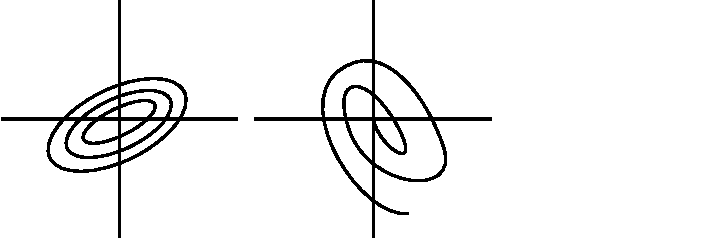
\includegraphics[scale=1.0]{../figures/centroyespiral.pdf}
\caption{Centro y Espiral.}
\end{figure}
\end{frame}

%\begin{frame}{Sistemas Lineales $\dot{X} = F(X)$ con $A$ singular}
%Cuando $A$ es una matriz 2x2 singular (no invertible) el comportamiento del sistema es ``especial'': existen una infinidad de puntos críticos $x \in \R^2$ además del origen y el retrato de fase del sistema debe ser equivalente a uno de los siguientes.
%
%\begin{figure} \centering
%    \includegraphics[scale=1.0]{../figures/amatriz0.pdf}  
%    \includegraphics[scale=1.0]{../figures/asingular_1.pdf}
%\end{figure}
%
%\end{frame}
%
%\begin{frame}{Sistemas Lineales $\dot{X} = F(X)$ con $A$ singular}
%\begin{figure} \centering
%    \includegraphics[scale=1.0]{../figures/asingular1.pdf}
%    \includegraphics[scale=1.0]{../figures/asingularr1.pdf}
%\end{figure}
%\end{frame}

\begin{frame}{Sistemas No Lineales y Linealización}
Si $\dot{X} = F(X)$ es un sistema no lineal entonces cerca de un punto crítico $X_0$ se tiene:
$$ \dot{X} = F(X) = DF(X_0)(X-X_0) + h(X),$$
donde $h(X) / (X-X_0) \to 0$ cuando $X \to X_0$. \\
\pause
``Pareciera'' entonces que en vecindad de $X_0$ podemos aproximar el sistema por

$$ \dot{X} = F(X) \approx DF(X_0)(X-X_0)$$

que, una vez aplicada una traslación, es un sistema lineal.\\ \pause
La idea es deducir de este sistema lineal (que se conoce bien) información acerca del sistema inicial. Veremos que esto no funciona bien en general.
\end{frame}

\begin{frame}{Sistemas No Lineales y Linealización - Ejemplo 1}
Consideremos el sistema

$$ \left\{ \begin{array}{l} \dot{x} = x^2 + y^2 - 6 \\ \dot{y} = x^2 - y \end{array} \right.. $$

En vecindad de $(-\sqrt{2}, 2)$ la versión linealizada es equivalente a

$$ \left\{ \begin{array}{l} \dot{x} = -2\sqrt{2}x + 4y \\ \dot{y} = -2\sqrt{2}x - y \end{array} \right.. $$
\end{frame}

\begin{frame}{Sistemas No Lineales y Linealización - Ejemplo 1}
\begin{figure}
	\includegraphics[scale=0.4]{figures/nonlinear-linealization.png} (a)
	\includegraphics[scale=0.4]{../figures/nolinealhiperbolico-espiral.png} (b)
	\caption{Retratos de fase: (a) Linealización (b) Sistema Original.}
\end{figure}
\end{frame}

\begin{frame}{Sistemas No Lineales y Linealización - Ejemplo 2}
Pensemos ahora en el sistema
$$ \left\{
	\begin{array}{l}
		\dot{x} = y + x(x^2 + y^2) \\
		\dot{y} = x + y(x^2 + y^2),
	\end{array} \right..
$$

cuya linealización cerca de $(0,0)$ es

$$ \left\{
	\begin{array}{l} \dot{x} = y \\ \dot{y} = -x \end{array} \right..
$$
\end{frame}

\begin{frame}{Sistemas No Lineales y Linealización - Ejemplo 2}
\begin{figure}
	\includegraphics[scale=0.4]{figures/nonlinear2-linealization.png} (a)
	\includegraphics[scale=0.4]{figures/nonlinear2.png} (b)
	\caption{Retratos de fase: (a) Linealización (b) Sistema Original.}
\end{figure}
\end{frame}

\begin{frame}{Sistemas No Lineales y Linealización}
Para sistemas no lineales la linealización es topológicamente equivalente al sistema original en vecindad de un punto crítico $X_0$ únicamente cuando la matriz Jacobiana $DF(X_0)$ tiene valores propios todos con parte real no nula.\\
Este es un teorema de \emph{Grobman} y \emph{Hartman}.
\end{frame}

\stframe{Teoría Avanzada:\\ Ciclos Límite y Teorema de Poincaré-Bendixson}

\begin{frame}{Ciclos Límite}
Ya hemos visto que en los retratos de fase pueden aparecer órbitas periódicas (ciclos) a los cuales tienden las demás órbitas cercanas, como ocurría en el Oscilador de Van der Pol:

\begin{figure}[!ht] \centering
	\includegraphics[scale=0.35]{../figures/vanderpol.png}
\end{figure}
\end{frame}

\begin{frame}{Ciclos Límite}
Este tipo de comportamiento que parece tan especial es, en realidad, típico de los sistemas planos, como lo garantiza el Teorema de Poincaré-Bendixson, uno de los resultados más fuertes de la teoría:

\begin{theorem}[Poincaré-Bendixson] Sea $F: \R^2 \to \R^2$ una función de clase $C^1$ y consideremos el sistema dinámico $\dot{X} = F(X)$.
Si $K$ es un subconjunto compacto del plano que no contiene puntos críticos (órbitas constantes) y hay alguna órbita $C$ dentro de $K$ entonces $C$ es un ciclo o tiende a un ciclo.
\end{theorem}
\end{frame}

\begin{frame}{Ciclos Límite}
\begin{itemize}
	\item El Teorema de Poincaré-Bendixson limita las posibilidades para las órbitas de un sistema dinámico plano.
	\item Es una consecuencia del Teorema de la Curva cerrada de Jordan y, por lo tanto, es aplicable únicamente a sistemas con estado de fases en $\R^2$.
	\item Todas las órbitas acotadas no triviales de un sistema plano deben ser ciclos o bien acercarse en el largo plazo ya sea a puntos críticos o a otros ciclos.
\end{itemize}

\end{frame}

\stframe{Teoría Avanzada:\\Bifurcaciones y Caos}
\begin{frame}{Bifurcaciones y Caos}
Otro comportamiento interesante que aparece en los sistemas dinámicos es el de bifurcación, que puede entenderse como el ``inicio del caos'': una bifurcación aparece cuando cambios (aún cuando sean muy pequeños) en los parámetros de un sistema resultan en diferencias importantes en su estructura topológica.\\ \pause
Formalmente, si el sistema $\dot{X} = F(\lambda, X)$ depende continuamente de un parámetro escalar $\lambda$ entonces existe $\lambda_0$ tal que la topología del retrato de fase cambia cuando $\lambda$ pasa por $\lambda_0$.
\end{frame}

\begin{frame}{Bifurcaciones y Caos}
Algunas bifurcaciones se refieren a cambios locales, alrededor de uno o varios puntos críticos:

\begin{figure} \centering
    \includegraphics[scale=0.9]{../figures/bifurcations-saddlenode.pdf}
    \caption{Bifurcación de silla-nodo.}	
\end{figure}
\end{frame}

\begin{frame}{Bifurcaciones y Caos}

\begin{figure} \centering
    \includegraphics[scale=0.9]{../figures/bifurcations-pitchforksupercritical.pdf} 
    \caption{Bifurcación \textit{pitchfork} supercrítica.}
\end{figure}
\end{frame}

\begin{frame}{Bifurcaciones y Caos}
Otras bifurcaciones se refieren a cambios globales en conjuntos más grandes como órbitas periódicas:
\begin{figure}[!ht] \centering
	\includegraphics[scale=0.2]{../figures/vanderpol-hopfbifurcation--0_1.png}
	\includegraphics[scale=0.2]{../figures/vanderpol-hopfbifurcation-0_0.png} \\
	\includegraphics[scale=0.2]{../figures/vanderpol-hopfbifurcation-0_1.png}
	\includegraphics[scale=0.2]{../figures/vanderpol-hopfbifurcation-0_3.png}
	\caption{Bifurcación de Poincaré-Andronov-Hopf en el oscilador de Van der Pol: $\lambda=-0.1;  0.0; 0.1; 0.3$}
\end{figure}
\end{frame}

% DYNAMITE
\section{DYNAMITE}
\stframe{DYNAMITE}
\begin{frame}{Generalidades}
DYNAMITE es una herramienta didáctica de \textbf{software libre} desarrollada por el autor para el estudio de sistemas dinámicos planos, los continuos en particular.
\end{frame}

\begin{frame}{Generalidades}
DYNAMITE está inspirado en \textit{Phaser}, aplicación propietaria que acompaña al libro ``Dynamics and Bifurcations`` de J. Hale y H. Ko\c{c}ak y que puede adquirirse también a través del sitio web \url{http://www.phaser.com}.
\end{frame}

\begin{frame}{Características}
Algunas de las características de DYNAMITE:

	\begin{itemize}
		\pause
		\item Es software libre: su distribución y modificación está permitida sin restricción alguna.
		\pause
		\item Puede ejecutarse (sin necesidad de software especial o \textit{plugins}) en cualquier navegador y, por ende, en cualquier plataforma (Mac OS X, Linux, Windows y móviles).
		\pause
		\item Produce gráficos vectoriales con calidad apta para publicación.
		\pause
		\item Soporta \textit{typesetting} de expresiones matemáticas utilizando MathML y ASCIIMath.
		\pause
		\item Tiene un diseño modular con dos integradores: Runge-Kutta combinado de orden 4-5 y ``backward Euler''.
	\end{itemize}
\end{frame}

\begin{frame}{Características}
	DYNAMITE está en capacidad de generar cualquiera de las siguientes gráficas:
	
	\begin{itemize}
		\pause
		\item Gráficas de funciones cartesianas $y = f(x)$ en una variable real.
		\pause
		\item Campos de pendientes $\vec{F}(x,y)$ asociados a un sistema dinámico plano $\dot{X} = \vec{F}(x,y)$.
		\pause
		\item Diagramas de fase con órbitas arbitrarias calculadas por DYNAMITE y con puntos iniciales definidos por el usuario.
		\pause
		\item Conjuntos de Julia asociados a sistemas dinámicos discretos obtenidos por iteración de polinomios cuadráticos complejos $f_c(z) = z^2 + c$, $z \in \C$.
	\end{itemize}
\end{frame}

\begin{frame}{Código Fuente y Descarga}
El código fuente de la última versión de DYNAMITE se encuentra disponible en línea en
$$ \text{\url{https://github.com/jorgeatorres/dynamite}}. $$
\pause
También allí pueden \sout{reportarse errores o comportamientos inesperados} colaborar con el proyecto.
\end{frame}

\begin{frame}{Ejemplos de uso}
\begin{enumerate}
\item Oscilador Armónico Lineal
\item Péndulo matemático
\item Modelo presa-depredador de Lotka-Volterra
\item Oscilador de Van der Pol
\end{enumerate}
\end{frame}

\begin{frame}{Ejemplos de uso}
\begin{example}[Otro sistema no lineal]
Construya el retrato de fase para sistema dinámico no lineal descrito por las ecuaciones:
$$
\left \{
	\begin{array}{ll}
		\dot{x} = y - y^3 \\
		\dot{y} = -x - y^2.
	\end{array} \right.
$$
\end{example}
\end{frame}

\begin{frame}{Ejemplos de uso - Conjuntos de Julia}
La iteración de funciones racionales complejas de la forma $f(z) = p(z) / q(z)$ define también un sistema dinámico plano en el cual las órbitas de cualquier punto se obtienen por composición:
$$ \gamma(z_0) = \{z_0, f(z_0), f\circ f(z_0), f \circ f \circ f(z_0), ..., f^k(z_0), ...\}. $$
El \emph{conjunto de Julia} de $f$ corresponde a la frontera del conjunto de puntos cuyas órbitas son no acotadas (i.e. $f^n(z_0) \to \infty$ cuando $n \to \infty$).
\end{frame}

%\begin{frame}{Ejemplos de uso - Conjuntos de Julia}
%Conjunto de Julia asociado a la función racional del método de Newton para hallar las raíces del polinomio cúbico $p(z) = z^3 - 1$:
%\begin{figure}[!ht] \centering
% \includegraphics[scale=0.1]{figures/juliaset-newton.png}
%\end{figure}
%\end{frame}

\begin{frame}{Ejemplos de uso - Conjuntos de Julia}
Conjunto de Julia asociado al polinomio $f_c(z) = z^2 + c$ con $c = 0.1 + 0.651i$.
\begin{figure}[!ht] \centering
 \includegraphics[scale=0.1]{figures/juliaset.png}
\end{figure}
\end{frame}

\begin{frame}{Licencia de DYNAMITE}
DYNAMITE está distribuído bajo licencia WTFPL (\textit{Do What The Fuck You Want To Public License}) cuyo inventor describe como
\begin{quote}``A very permissive license for software and other scientific or artistic works that offers a great degree of freedom''.
\end{quote}
\end{frame}

\section{Fin}
\stframe{Gracias por su atención.}

\begin{frame}
\begin{figure} \centering
\includegraphics[scale=0.2]{figures/thats-all-folks.jpg}
\end{figure}
\end{frame}


\end{document}